
\part{Vorbereitung\label{part:Vorbereitung}}

\chapter{Motivationsbeispiele\label{chap:Einleitung}}

Dieses Kapitel befasst sich mit der Modellierung einiger technischer
Beispielsysteme, bei denen man auf nichtlineare Modellgleichungen
geführt wird. Auf diese Beispielsysteme wird in den weiteren Kapiteln
mehrfach zurückgegriffen.

\section{Mobiler Roboter\label{subsec:Mobiler-Roboter-Modellierung}}

Mobile Roboter spielen eine wichtige Rolle bei der automatisierten
Lagerhaltung und bei flexiblen Fertigungsprozessen, finden aber auch
als Inspektions- bzw. Serviceroboter Anwendung. Abb.~\ref{fig:mobiler-roboter-kinematisches-modell}~(links)
stellt einen für Lehrzwecke entwickelten mobilen Roboter mit zwei
Rädern dar~\cite{roebenack2015roboter}.

\begin{figure}
\begin{centering}
\begin{tabular}{ccc}
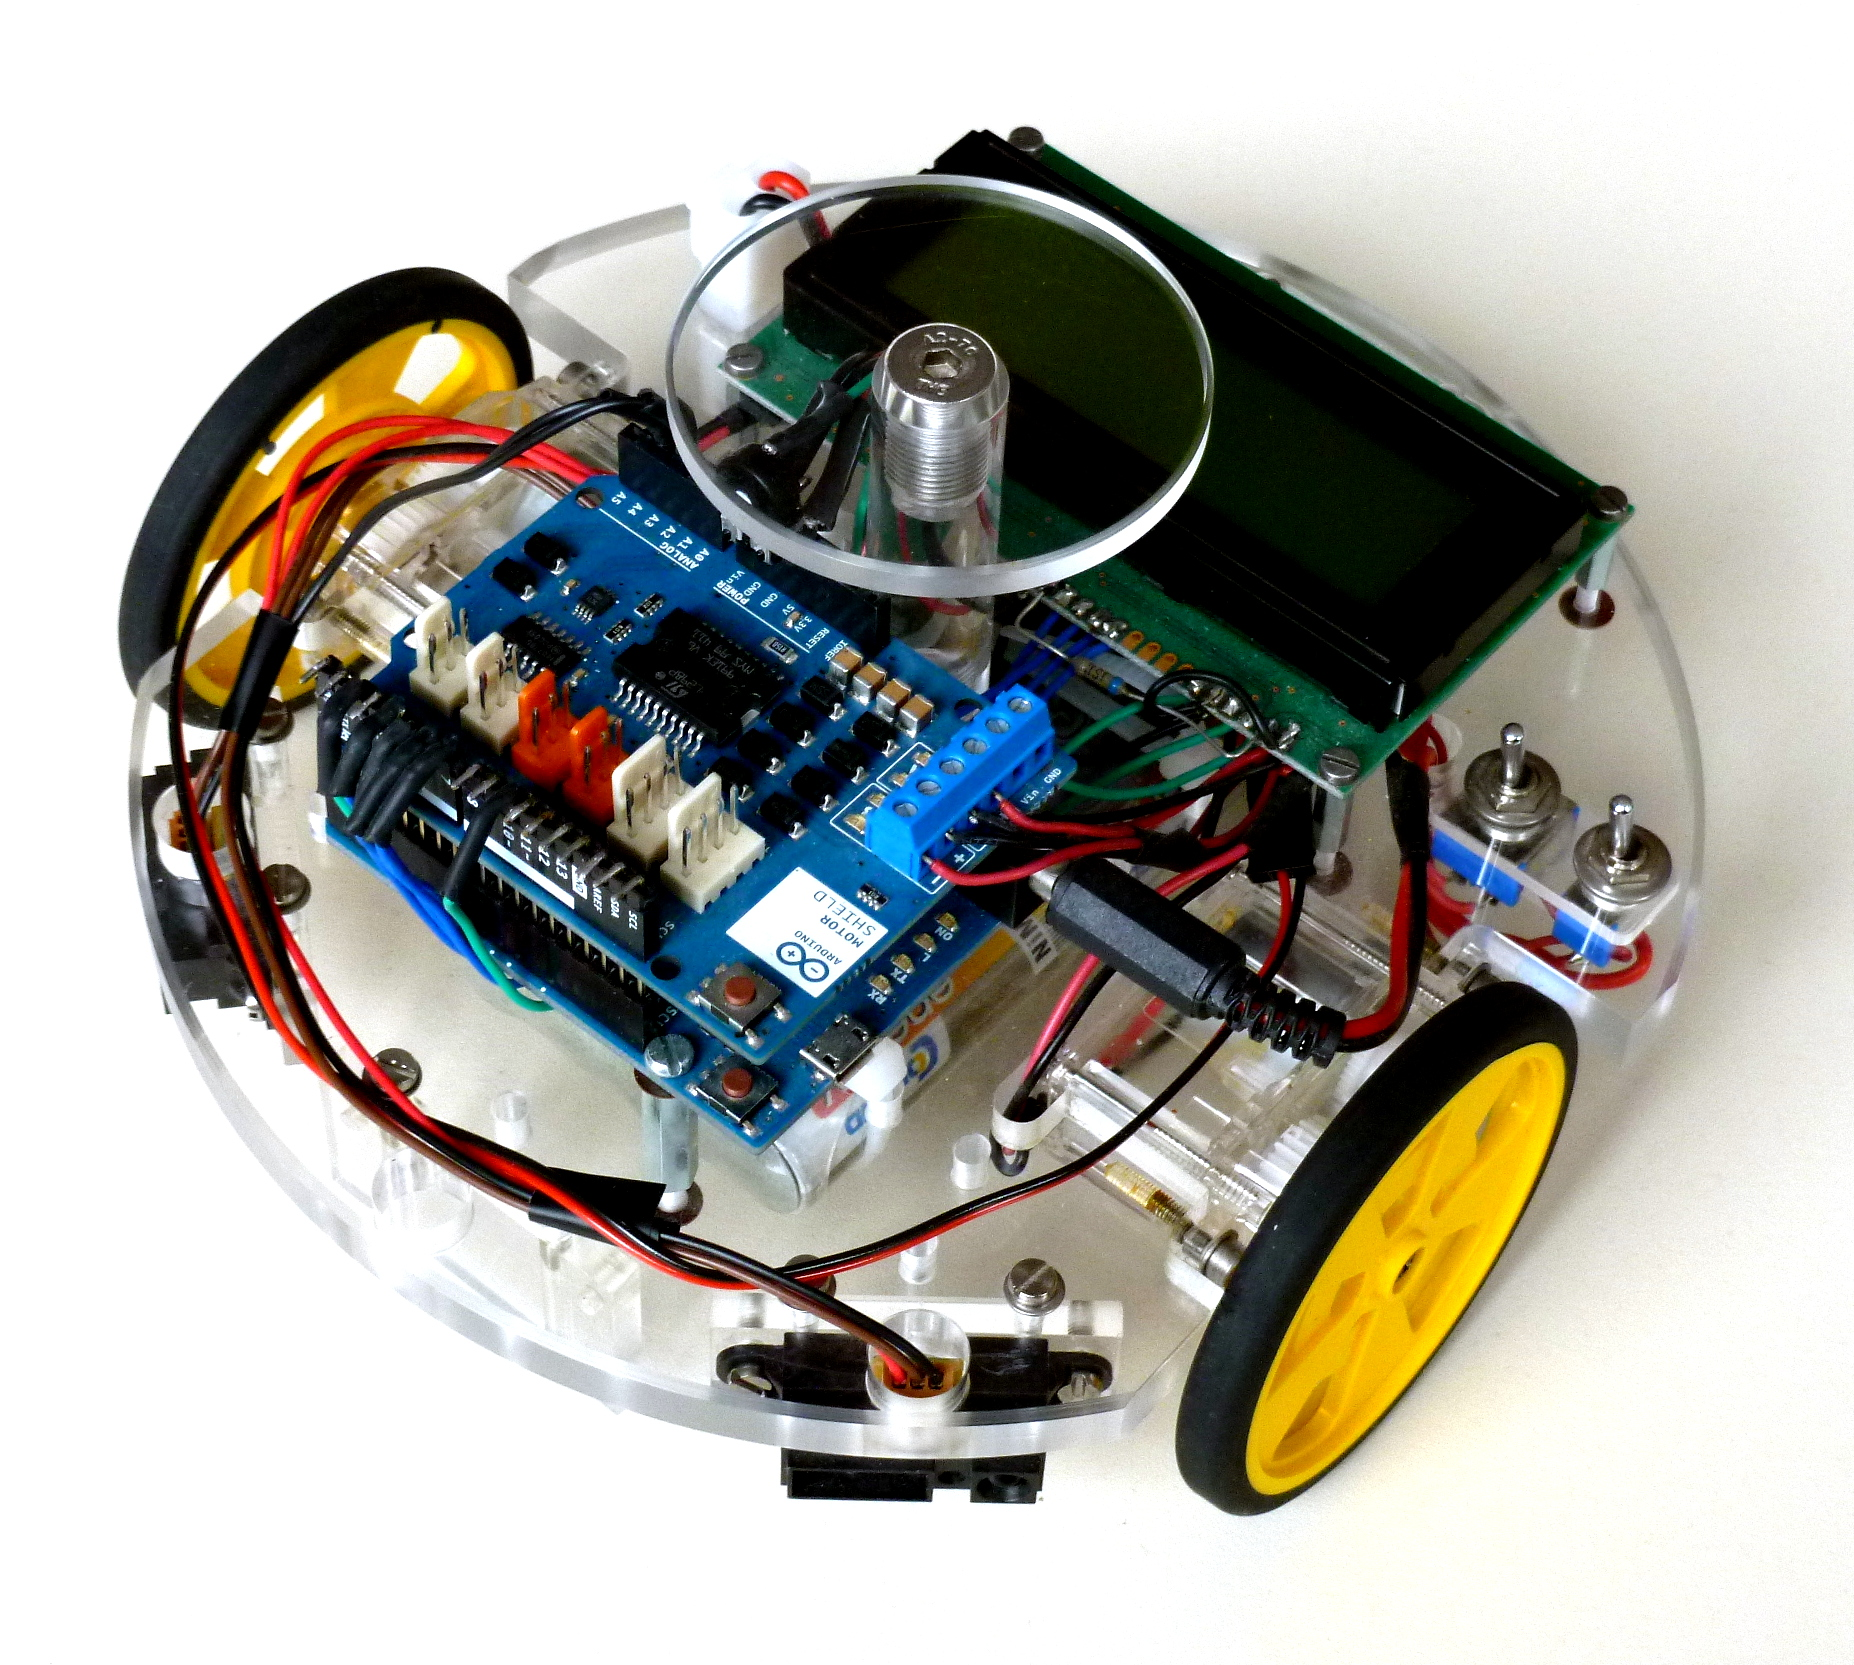
\includegraphics[width=0.45\textwidth]{Roboter_Foto} & \hspace*{0.05\textwidth} & 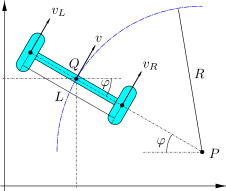
\includegraphics[width=0.45\textwidth]{Roboter_kin_Modell}\tabularnewline
\end{tabular}
\par\end{centering}
\caption{Mobiler Roboter, Prototyp nach~\cite{roebenack2015roboter} (links),
Modell in der $(x_{1},x_{2})$-Ebene (rechts)\label{fig:mobiler-roboter-kinematisches-modell}}
\end{figure}

Für den mobilen Roboters wird nachfolgend ein kinematisches Modell
hergeleitet. Dieses Modell beschreibt die Bewegung in der Ebene ohne
Berücksichtigung der die Bewegung verursachenden Kräfte. Der Antrieb
des Roboters erfolgt über zwei Räder mit dem Radius~$r$. Das linke
Rad habe die Winkelgeschwindigkeit $\omega_{L}$, das rechte die Winkelgeschwindigkeit
$\omega_{R}$. An den Auflagepunkten der Räder erhält man die Tangentialgeschwindigkeiten
\[
\begin{array}{lcl}
v_{L} & = & \omega_{L}r,\\
v_{R} & = & \omega_{R}r.
\end{array}
\]
Für unterschiedliche Winkelgeschwindigkeiten (also $\omega_{L}\neq\omega_{R}$)
dreht sich der Roboter. Wir stellen uns diese Drehung als Umfahrung
eines (fiktiven) Punktes~$P$ vor, der zum Mittelpunkt~$Q$ des
Roboters den Abstand~$R$ habe. Linkes und rechtes Rad haben von
dem Punkt~$P$ die Abstände
\[
\begin{array}{lcl}
R_{L} & = & R+\frac{L}{2},\\
R_{R} & = & R-\frac{L}{2},
\end{array}
\]
wobei~$L$ den Abstand beider Räder voneinander bezeichnet. Beschreibt
man die Rotation um den Punkt~$P$ mit dem in Abb.~\ref{fig:mobiler-roboter-kinematisches-modell}~(rechts)
eingeführten Winkel~$\varphi$, so erhält man die Rotationgeschwindigkeit
\begin{equation}
\omega=\dot{\varphi}\label{eq:roboter-modell-rot}
\end{equation}
als zeitliche Ableitung des Winkels. Zu den Tangentialgeschwindigkeiten
der beiden Räder besteht dann der Zusammenhang
\[
\begin{array}{lcl}
v_{L} & = & \omega R_{L},\\
v_{R} & = & \omega R_{R}.
\end{array}
\]
Aus gegebenen Winkelgeschwindigkeiten~$\omega_{L}$ und~$\omega_{R}$
der Motoren kann man damit einerseits die Rotationsgeschwindigkeit
des Roboters um die eigene Achse bestimmen
\[
\omega=\frac{r}{L}\left(\omega_{L}-\omega_{R}\right),
\]
andererseits auch den Abstand
\[
R=\frac{L}{2}\left(\frac{\omega_{L}+\omega_{R}}{\omega_{L}-\omega_{R}}\right)
\]
zwischen dem Punkt~$Q$ und dem Drehpunkt~$P$. Damit erhält man
zugleich die translatorische Geschwindigkeit 
\[
v=\omega R=\frac{r}{2}\left(\omega_{L}+\omega_{R}\right)
\]
des Roboters. Mit dem Winkel~$\varphi$ und der Geschwindigkeit~$v$
lässt sich die translatorische Bewegung beschreiben: 
\begin{equation}
\begin{array}{lcl}
\dot{x}_{1} & = & v\,\sin\varphi,\\
\dot{x}_{2} & = & v\,\cos\varphi.
\end{array}\label{eq:roboter-modell-trans}
\end{equation}
Führt man den Zustand 
\[
x=\left(\begin{array}{c}
x_{1}\\
x_{2}\\
x_{3}
\end{array}\right)=\left(\begin{array}{c}
x_{1}\\
x_{2}\\
\varphi
\end{array}\right)
\]
sowie die Eingänge $u_{1}=v$ und $u_{2}=\omega$ ein, so liefert
die Kombination aus~(\ref{eq:roboter-modell-rot}) und~(\ref{eq:roboter-modell-trans})
das kinematische Gesamtmodell 
\begin{equation}
\left(\begin{array}{c}
\dot{x}_{1}\\
\dot{x}_{2}\\
\dot{x}_{3}
\end{array}\right)=\left(\begin{array}{c}
\sin x_{3}\\
\cos x_{3}\\
0
\end{array}\right)u_{1}+\left(\begin{array}{c}
0\\
0\\
1
\end{array}\right)u_{2}.\label{eq:roboter-kinematisches-modell}
\end{equation}
Bedingt durch die Winkelfunktionen liegt damit ein Modell als nichtlineares
Differentialgleichungssystem vor. Genauer gesagt ist das Modell~(\ref{eq:roboter-kinematisches-modell})
nichtlinear bezüglich des Zustands~$x$, aber linear hinsichtlich
der Eingänge~$u_{1}$ und~$u_{2}$.

Das kinematische Robotermodell~(\ref{eq:roboter-kinematisches-modell})
lässt sich als einachsiges Fahrzeugmodell aufgefassen. Kinematische
Fahrzeugmodelle werden auch bei aktuellen Forschungsvorhaben genutzt,
beispielsweise bei der Spurregelung und beobachterbasierten Spurschätzung
für mehrachsige, mehrgliedrige bzw. mehr\-achs\-gelenkte Fahrzeuge
(LKWs, LKWs mit Anhänger, überlange Beförderungssysteme wie z.\,B.
AutoTram\textsuperscript{\textregistered}, siehe \cite{huber2012ssd,nitzsche2014ecc,riesmeier2016}).

\section{Wagen mit Pendel\label{subsec:Wagen-mit-Pendel}}

Verladebrücken bzw. Brückenkräne werden in Montagehallen, in Lagern
und auf Güterumschlagplätzen (z.\,B. Güterbahnhöfen, Häfen) eingesetzt.
Für eine schnelle Bewegung bzw. hochpräzise Positionierung der zu
transportierenden Lasten ist eine Regelung erforderlich.

Aus physikalischer Sicht kann man eine Verladebrücke als ein horizontal
bewegliches Pendel auffassen. Abb.~\ref{fig:Wagen-mit-Pendel} zeigt
einen Wagen, an welchem ein Pendel der Länge~$\ell$ angebracht ist.
Zur Vereinfachung gehen wir von einer festen Seillänge~$\ell$ aus.
Der Wagen habe die Masse~$m_{1}$, die Last die Masse~$m_{2}$.
Das Seil selber werde als masselos angenommen. Die Lage des Systems
wird durch die Wagenposition~$q_{1}$ und den Pendelwinkel~$q_{2}$
beschrieben. Eine auf den Wagen wirkende Kraft~$\digamma$ stellt
den Eingang des Wagen-Pendel-Systems dar.

\begin{figure}
\begin{centering}
\resizebox{0.5\textwidth}{!}{\input{wagen_pendel.pdftex_t}}
\par\end{centering}
\caption{Wagen mit Pendel\label{fig:Wagen-mit-Pendel}}

\end{figure}

Die kinetische Energie hat die Form
\[
T=\frac{m_{1}}{2}\dot{q}_{1}^{2}+\frac{m_{2}}{2}\left(\dot{x}_{s}^{2}+\dot{y}_{s}^{2}\right),
\]
wobei die Position der Last durch die Koordinaten 
\begin{eqnarray*}
x_{s} & = & q_{1}+\ell\sin q_{2}\\
y_{s} & = & \ell\cos q_{2}
\end{eqnarray*}
beschrieben wird. Daraus ergibt sich unmittelbar 
\[
T=\frac{m_{1}+m_{2}}{2}\dot{q}_{1}^{2}+m_{2}\ell\dot{q}_{1}\dot{q}_{2}\cos q_{2}+\frac{m_{2}}{2}\ell^{2}\dot{q}_{2}^{2}.
\]
Mit der potentiellen Energie 
\[
V=m_{2}g\ell(1-\cos q_{2})
\]
erhält man die Lagrange-Funktion $L=T-V$. Die Bewegungsgleichungen
haben die Form
\[
M(q)\ddot{q}+C(q,\dot{q})+K(q)=Q
\]
mit der Massematrix 
\[
M(q)=\left(\begin{array}{cc}
m_{1}+m_{2} & \ell m_{2}\cos q_{2}\\
\ell m_{2}\cos q_{2} & \ell^{2}m_{2}
\end{array}\right).
\]
Die Vektoren~$C$ und~$K$ beinhalten die Zentrifugal- und Corioliskräfte
bzw. die Potentialkräfte 
\[
C(q,\dot{q})=\left(\begin{array}{c}
-\ell m_{2}\dot{q}_{2}^{2}\sin q_{2}\\
\text{0}
\end{array}\right),\quad K(q)=\left(\begin{array}{c}
0\\
m_{2}g\ell\sin q_{2}
\end{array}\right).
\]
Als äußere Kräfte wirken die Reibungskräfte (viskose Reibung mit den
Koeffizienten~$d_{1}$ und~$d_{2}$) sowie die auf den Wagen eingeprägte
Kraft~$\digamma$:
\[
Q=\left(\begin{array}{c}
\digamma-d_{1}\dot{q}_{1}\\
-d_{2}\dot{q}_{2}
\end{array}\right).
\]
Mit dem Zustand $x=(q_{1},\dot{q}_{1},q_{2},\dot{q}_{2})^{T}$ und
dem Eingang $u=\digamma$ erhält man das folgende nichtlineare Modell:
\begin{equation}
\begin{array}{lcl}
\dot{x}_{1} & = & x_{2}\\
\dot{x}_{2} & = & \frac{m_{2}\ell^{2}x_{4}^{2}\sin x_{3}-d_{1}\ell x_{2}+\cos x_{3}\left(m_{2}g\ell\sin x_{3}+d_{2}x_{4}\right)+\ell u}{\ell\left(m_{1}+m_{2}\sin^{2}x_{3}\right)}\\
\dot{x}_{3} & = & x_{4}\\
\dot{x}_{4} & = & \frac{-\left(m_{1}+m_{2}\right)\left(m_{2}g\ell\sin x_{3}+d_{2}x_{4}\right)-\cos x_{3}\left(\ell^{2}m_{2}^{2}x_{4}^{2}\sin x_{3}-d_{1}\ell m_{2}x_{2}\right)-\ell m_{2}u\cos x_{3}}{\ell^{2}m_{2}\left(m_{1}+m_{2}\sin^{2}x_{3}\right)}
\end{array}\label{eq:modell-pendel-mit-wagen}
\end{equation}
Das Modell ist nichtlinear im Zustand~$x$, aber affin im Eingang~$u$.

\section{Hochsetzsteller\label{subsec:Hochsetzsteller-Modellierung}}

Mit Spannungswandlern lassen sich verschiedene Spannungsniveaus aneinander
anpassen, z.\,B. zwischen einer bereitgestellten Versorgungsspannung
und einem Verbraucher. Gleichsspannungswandler sind ein beliebte Objekte
für die Erprobung und den Vergleich nichtlinearer Regelungsverfahren~\cite{sira-ramirez1991ijc,kugi2000at,gensior2006}.
Aufgrund ihres Wirkungsgrades werden geschaltete Spannungswandler
in vielen Bereichen der Leistungselektronik und der Antriebstechnik
eingesetzt.

Ein \emph{Hochsetzsteller}\index{Hochsetzsteller} bzw. \emph{Aufwärtswandler}
(engl. \emph{Boost Converter}) ist ein Gleichspannungswandler, der
eine Eingangsspannung in eine höhere Ausgangsspannung überführt~\cite{erickson2004,bacha2014}.
Das Schaltbild in Abb.~\ref{fig:hochsetzsteller-schaltbild-netzwerk}
zeigt die grundsätzliche Schaltungstopologie bzw. das Netzwerkmodell
eines Hochsetzstellers. Der Leistungstransistor wird zusammen mit
der Freilaufdiode als Umschalter modelliert, wobei $d=1$ einem durchgesteuerten
Transistor und $d=0$ einem sperrenden Transistor entspricht. 

\begin{figure}
\begin{centering}
\resizebox{0.99\textwidth}{!}{\input{schaltbild-boost-konverter.pdftex_t}}
\par\end{centering}
\caption{Prinzipschaltbild (links) und Netzwerkmodell (rechts) eines Hochsetzstellers\label{fig:hochsetzsteller-schaltbild-netzwerk}}

\end{figure}
Für den Spulenstrom~$I$ gilt aufgrund des Maschensatzes 
\[
L\dot{I}=E+\left\{ \begin{array}{rcl}
0 & \text{für} & d=1,\\
-U & \text{für} & d=0.
\end{array}\right.
\]
Die Bilanzierung der in den Kondensator fließenden Ströme (Knotensatz)
liefert 
\[
C\dot{U}=-\frac{U}{R}+\left\{ \begin{array}{rcl}
0 & \text{für} & d=1,\\
I & \text{für} & d=0.
\end{array}\right.
\]
Mit Einführung des Vektors $x=(x_{1},x_{2})^{T}=(I,U)^{T}$ erhält
man das Differentialgleichungssystem 
\begin{equation}
\begin{array}{lcl}
\dot{x}_{1} & = & -(1-d)\frac{1}{L}x_{2}+\frac{E}{L},\\
\dot{x}_{2} & = & (1-d)\frac{1}{C}x_{1}-\frac{1}{RC}x_{2}.
\end{array}\label{eq:Hochsetzsteller-modell}
\end{equation}
Das System ist aufgrund der Produktbildung zwischen dem Eingang~$d$
und den Komponenten des Zustands~$x$ nichtlinear. Ein solches Modell
nennt man auch bilinear~\cite{schwarz91}.

Der Eingang~$d$ beschreibt das Verhalten des als Schalter modellierten
Transistors und kann zunächst nur die diskreten Werte $d\in\{0,1\}$
annehmen. In diesem Kontext liegt mit Gl.~(\ref{eq:Hochsetzsteller-modell})
ein \emph{geschaltetes Modell} (engl. \emph{switched model}) vor.
Mit einer \emph{Pulsweitenmodulation} (kurz \emph{PWM}, engl. \emph{pulse
width modulation}) lassen sich auch Zwischenwerte einstellen (siehe
Abb.~\ref{fig:PWM}). Das Verhältnis der Einschaltzeit mit $d=1$
gegenüber der Schaltperiode $T>0$ bezeichnet man dabei als as \emph{Tastverhältnis~}$\bar{d}$
(engl. \emph{duty ratio}), welches Werte aus dem Intervall $\bar{d}\in[0,1]$
annehmen kann.

\begin{figure}
\begin{centering}
\resizebox{0.55\textwidth}{!}{\input{PWM.pdftex_t}}
\par\end{centering}
\caption{Signalverlauf des Eingangs~$d$ bei Pulsweitenmodulation (PWM)\label{fig:PWM}}
\end{figure}

Das Tastverhältnis~$\bar{d}$ gibt den Mittelwert des Schaltsignals~$d$
über eine Periode~$T$ an:
\[
\bar{d}(t)=\frac{1}{T}\int_{t}^{t+T}d(\tau)\,\d\tau.
\]
In analoger Weise kann man auch für alle anderen Systemgrößen (Ströme,
Spannungen, ggf. Ladungen usw.) gemittelte Größen einführen. In diesem
Sinne erhält man mit 
\[
\bar{x}_{i}(t)=\frac{1}{T}\int_{t}^{t+T}x_{i}(\tau)\,\d\tau\quad\text{für}\quad i=1,2
\]
die gemittelten Zustandskomponenten aus dem Modell~(\ref{eq:Hochsetzsteller-modell}).
Der zeitliche Verlauf der gemittelten Größen lässt sich wiederum durch
ein Differentialgleichungssystem beschreiben. Für den Grenzübergang
$T\to0$, was aus technischer Sicht durch eine hinreichend hohe Schaltfrequenz
$1/T$ angenähert wird, erhält man für die gemittelten Größen das
\emph{gemittelte Modell} (engl. \emph{averaged model}):
\begin{equation}
\begin{array}{lcl}
\dot{\bar{x}}_{1} & = & -(1-\bar{d})\frac{1}{L}\bar{x}_{2}+\frac{E}{L}\\
\dot{\bar{x}}_{2} & = & (1-\bar{d})\frac{1}{C}\bar{x}_{1}-\frac{1}{RC}\bar{x}_{2}.
\end{array}\label{eq:Hochsetzsteller-modell-gemittelt}
\end{equation}
Das gemittelte Modell~(\ref{eq:Hochsetzsteller-modell-gemittelt})
in seiner Struktur vollständig mit dem Modell~(\ref{eq:Hochsetzsteller-modell})
übereinstimmt, wird man in der praktischen Handhabung darauf verzichten,
die gemittelen Größen separat auszuweisen. Den Reglerentwurf führt
man an dem (hinsichtlich des Eingangssignals wertkontunierlichen)
gemittelten Modell durch, bei der Implementierung wird das Reglerausgangssignal
nach einer Pulsweitenmodulation dem geschalteten System zugeführt.

\bibliographystyle{babalpha}
\bibliography{dynamic}

